\begin{figure}[htbp]
	% Partly taken from http://www.texample.net/tikz/examples/convolution-of-two-functions/
	\centering
	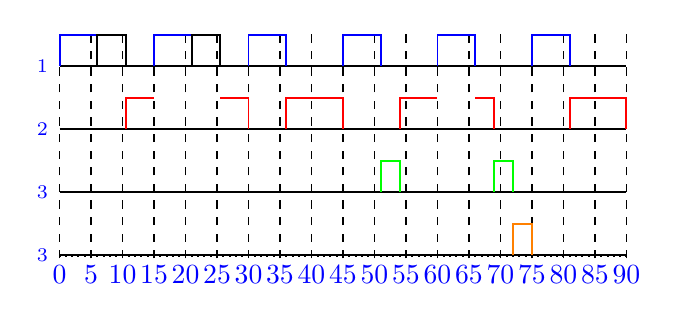
\begin{tikzpicture}[
		scale=0.08,
		line width=0.25mm,
		every node/.style={scale=1, text=blue},
		major tick/.style={semithick, dashed},
		x tick label/.style={anchor=north, minimum width=5mm},
		task1/.style={blue},
		task2/.style={red},
		task3/.style={green},
		task4/.style={orange},
		overload/.style={black},
		desc/.style={anchor=east}
		]

	% Task 4
	\draw (0, 0) -- (90, 0);
	\node[desc] at (0, 0) {$\uptau_3$};

	% Task 3
	\draw (0, 10) -- (90, 10);
	\node[desc] at (0, 10) {$\uptau_3$};
	
	% Task 2
	\draw (0, 20) -- (90, 20);
	\node[desc] at (0, 20) {$\uptau_2$};	

	% Task 1
	\draw (0, 30) -- (90, 30);
	\node[desc] at (0, 30) {$\uptau_1$};	

	
	% Small ticks
	\foreach \x in {0, 1,...,90}{
		\draw (\x, -0.25) -- (\x, 0.25);
	}
	
	% Major ticks with label
	\foreach \x/\label in {0, 5,...,90}{
		\node[x tick label] at (\x, 0) {$\label$}; 		
		\draw[major tick] (\x, -0.5) -- (\x, 36);
	}
	
	% Draw all
	\foreach \x in {0, 15,...,89}{
		\draw[task1] (\x, 30) -- (\x, 35) -- (\x+6, 35) -- (\x+6, 30);
	}

	\draw[overload] (6, 30) --  (6, 35) --  (10.5, 35) -- (10.5, 30);
	\draw[task2] (10.5, 20) -- (10.5, 25) -- (15, 25); % Done: 4.5 von 9
	\draw[overload] (21, 30) --  (21, 35) --  (25.5, 35) -- (25.5, 30);
	\draw[task2] (25.5, 25) -- (30, 25) -- (30, 20); % Deadline miss
	\draw[task2] (36, 20) -- (36, 25) -- (45, 25) -- (45, 20);
	\draw[task3] (51, 10) -- (51, 15) -- (54, 15) -- (54, 10);
	\draw[task2] (54, 20) -- (54, 25) -- (60, 25);
	\draw[task2] (66, 25) -- (69, 25) -- (69, 20);
	\draw[task3] (69, 10) -- (69, 15) -- (72, 15) -- (72, 10);
	\draw[task4] (72, 0) -- (72, 5) -- (75, 5) -- (75, 0);
	\draw[task2] (81, 20) -- (81, 25) -- (90, 25) -- (90, 20);
			
	\end{tikzpicture}
%	\caption{Ablaufübersicht}
\end{figure} 